\chapter{Concepto de Medida}%
En general, la teoría de la integración está sustentada mayoritariamente por el concepto de medida que se tiene en el espacio sobre el que se integra. Pueden darse dos situaciones, que se defina una medida y a partir de ahí la integral correspondiente o puede ocurrir que se defina la integral y a partir de la misma se mida. Nosotros optaremos por definir todo lo relativo a la medida de forma previa, para que la teoría de integración que se desarrollará después esté sustentada en las propiedades métricas con las que dotemos a $\mathbb{R}^n$ y que caracterizarán la teoría posterior.

\section{Medida}
El concepto fundamental de esta sección es comprender qué entendemos por medida y que propiedades tiene, así como demostrar que la medida de Lebesgue es un buen instrumento de medida para trabajar en $\mathbb{R}^n$.

\begin{defi}[Medida]
Sea una $\sigma$-álgebra $\left( X, M \right)$, una \textbf{medida positiva} será $\mu: M \rightarrow \overline{\mathbb{R}^+} \cup \{0\}$ tal que:
\begin{itemize}
    \item $\mu\left( \emptyset \right) = 0$
    \item $\mu\left( \bigcup_{j = 1}^{\infty} A_j \right) = \sum_{i=1}^{\infty} \mu \left( A_j \right)\quad A_j \cap A_i = \emptyset,\ \forall i \neq j$. (\textbf{$\sigma$ aditividad})
\end{itemize}
\end{defi}

\begin{defi}[Rectángulo]
Definimos un rectángulo en $\mathbb{R}^n$ como el conjunto;
$$Q = \left[ a_1, b_1 \right] \times \ldots \times \left[ a_n, b_n \right] \subset \mathbb{R}^{n}$$
Además, definimos como \textbf{volumen} de $Q$ a 
$$v\left( Q \right) = \left( b_n - a_n \right) \cdots \left( b_1 - a_1 \right)$$
\end{defi}

\begin{defi}[Medida exterior de Lebesgue]
Sea $A \subset \mathbb{R}^{n}$, definimos como \textbf{medida exterior} de $A$ a:
$$
\mu^{*}(A) = \inf \sum_{k=1}^{\infty} v\left( Q_k \right); \text{ donde } \{Q_k\}_{k=1}^{\infty} \text{ y } A \subset \bigcup_{k = 1}^{\infty} Q_k
$$ 
\end{defi}

\begin{obs}
Podemos restringir las familias $\{Q_k\}$ a aquellas que tengan $\mathrm{diam}\ Q_k < \delta$ para un cierto delta y la definición no cambia. Esto es así porque, en el fondo, el conjunto de sumatorios de volúmenes que estamos escogiendo es el mismo, ya que para familias con algún $Q_k$ de diámetro mayor, éste se puede dividir en varios rectángulos más pequeños cuyo volumen suman el de $Q_k$ pero cuyo diámetro es menor que dicho delta.
\end{obs}

\begin{defi}[Medida nula]
Decimos que $A$ tiene medida nula si podemos encontrar recubrimientos de $A$ con sumatorio de volúmenes tan pequeños como queramos, es decir:
$$\mu^{*}\left( A \right) = 0 \Leftrightarrow \forall \varepsilon > 0 \ \exists \{Q_k\} \text{ rec. de } A: \sum_{k=1}^{\infty} v\left( Q_k \right) < \varepsilon $$  
\end{defi}

\begin{ej}
	\begin{enumerate}
       \item Si $x_0 \in \mathbb{R}^{n}$, entonces $\forall \varepsilon > 0, \exists k \in \mathbb N: \ v\left( Q\left( x_0 \right)  \right) < \frac{\varepsilon}{2^{k}}$, luego es de medida nula.
       \item Si $N$ numerable, entonces podemos escribir $N = \{x_k\}$, para cada $x_k$ podemos encontrar $Q_k\left( x_k \right): v\left( Q_k\left( x_k \right)  \right) < \frac{\varepsilon}{2^{k}}$ que lo contenga, luego se tiene que es de medida nula.
    \end{enumerate}
\end{ej}
    
\begin{prop}
La medida exterior de Lebesgue cumple las siguientes propiedades:
\begin{itemize}
\item \textbf{Invariante por traslaciones}:
$$A \subset \mathbb{R}^{n}, \ c \in \mathbb{R}^{n} \Rightarrow \mu^{*}\left( c + A \right) = \mu^{*}\left( A \right) $$ 
\item \textbf{Covariante con respecto a la inclusión}:
$$A \subset B \subset \mathbb{R}^{n} \Rightarrow \mu^{*}\left( A \right) \le \mu^{*}\left( B \right) $$
\item \textbf{Semiaditiva}:
$$A,\ B \in \mathbb{R}^{n} \Rightarrow \mu^{*}\left( A \cup B \right) \le \mu^{*}\left( A \right) + \mu^{*}\left( B \right)$$
\end{itemize}
\end{prop}
\begin{demo}
\begin{itemize}
\item Trivial

\item Si $\mu^{*}\left( B \right) = +\infty$ es trivial, luego suponemos que no.

Sea $\{Q_k\}$ un recubrimiento de $B$, como $A \subset B \Rightarrow \{Q_k\}$ es un recubrimiento de A, luego\footnote{Puesto que si eres menor que todos los elementos de un conjunto eres menor o igual que su ínfimo.}
$$\forall \{Q_k\}: \mu^{*}\left( A \right) < \sum_{k=1}^{\infty} v\left( Q_k \right) \Rightarrow \mu^{*}\left( A \right) \le \mu^{*}\left( B \right) $$

\item Si $\mu^{*}\left( A \right) = +\infty$ o $\mu^{*}\left( B \right) = +\infty$ es trivial. 
 
Suponiendo ambos finitos, entonces para $\varepsilon > 0$ se tiene que:
$$\begin{cases}
\exists \{Q_k\} \text{ rec. de A: } \sum_{k=1}^{\infty} v\left( Q_k \right) < \mu^{*}\left( A \right) + \frac{\varepsilon}{2}  \\
\exists \{R_k\} \text{ rec. de B: } \sum_{k=1}^{\infty} v\left( R_k \right) < \mu^{*}\left( A \right) + \frac{\varepsilon}{2} 
\end{cases}
$$
Consideremos $ \{Q_k, R_k\} = \{S_j\}$ donde $S_j = \begin{cases}
Q_{\frac{j}{2}},\ j \text{ par} \\
R_{\frac{j+1}{2}},\ j \text{ impar} 
\end{cases}$. Tenemos trivialmente que $\{S_j\}$ es rec. de $A\cup B$, luego:
$$\mu^{*}\left( A\cup B \right) \le \sum_{j=1}^{\infty} v\left( S_j \right) = \sum_{k=1}^{\infty} v\left( Q_k \right) + \sum_{k=1}^{\infty} v\left( R_k \right) < \mu^{*}\left( A \right) + \mu^{*}\left( B \right) + \varepsilon$$
Y como dicha desigualdad es para cualquier $\varepsilon > 0$ se tiene la desigualdad del enunciado.
\end{itemize}
\end{demo}

\begin{prop}
En cualquier rectángulo, la medida exterior y su volumen coinciden, esto es:
$$\forall Q \subset \mathbb{R}^n : v\left( Q \right) = \mu^{*}\left( Q \right)$$
\end{prop}
\begin{demo}
    \begin{itemize}
        \item $ \mu^*\left( Q \right) \le v\left( Q \right) $:
        
        Tomamos $\varepsilon > 0$ y consideramos la familia $ \{Q_k\}$ recubrimiento de $Q$ donde $Q_1 = Q$ y $\forall k \geq 2 : v(Q_k) < \varepsilon/2^{k}$. De este modo, $\{Q_k\} $ es rec. de $Q$ y además
$$\sum_{k=1}^{\infty} v\left( Q_k \right) = v\left( Q \right) + \sum_{k=2}^{\infty} v\left( Q_k \right) < v\left( Q \right) + \sum_{k=2}^{\infty} \frac{\varepsilon}{2^{k}} < v\left( Q \right) + \varepsilon$$
		Por tanto, por ser ínfimo y ser para todo epsilon, se tiene:
		$$\mu^*\left( Q \right) \le v\left( Q \right) + \varepsilon \Rightarrow \mu^*\left( Q \right) \le v\left( Q \right)$$
        \item $v\left( Q \right) \le \mu^*\left( Q \right)$:
        
        Observamos que $ \overline{Q}$ es la unión de las caras de $Q$ que denotaremos por $C_i$, por tanto:
        \begin{align*}
        v\left( Q \right) = v\left( \overline{Q} \right)  && \mu^{*}\left( Q \right) \le \mu^{*}\left( \overline{Q} \right)
        \end{align*}
        $$\mu^{*}\left( \overline{Q} \right) = \mu^{*}\left( Q \cup \left( C_1, \ldots, C_m \right)  \right) \le \mu^{*}\left( Q \right) + \mu^{*}\left( C_1 \right) + \ldots + \mu^{*}\left( C_m \right) = \mu^{*}\left( Q \right)$$
        Luego, concluimos que un cubo cualquiera tiene la misma medida que el mismo cubo, pero cerrado. Por tanto, podemos suponer que $Q$ es cerrado y por ser acotado en $\mathbb{R}^n$ es compacto. 
        
Si el volumen es menor que todos los posibles sumatorios, entonces tendrá que ser menor que el ínfimo, luego basta probar que $v\left( Q \right) \le \sum_{k=1}^{\infty} v\left( Q_k \right), \ \forall \{Q_k\} \ Q \subset \bigcup_{k \in \mathbb{N}} Q_k $.

Como $Q$ lo podíamos considerar compacto, se tiene que dado un recubrimiento $\{Q_k\}_{k=1}^{\infty}$:
$$Q \subset Q_1 \cup \ldots \cup Q_N \Rightarrow v\left( Q \right) \le v\left( Q_1 \right) +\ldots+v\left( Q_N \right) \le \sum_{k=1}^{\infty} v\left( Q_k \right)$$
\end{itemize}
\end{demo}

\begin{defi}
Definimos el \textbf{diámetro de un conjunto} como:
$$\mathrm{diam}\ A = \sup \{\vert \vert x - y \vert  \vert: \ x,y \in A\}$$
Y definimos la \textbf{distancia entre dos conjuntos} como:
$$d(A,B) = \inf \{||x-y||: x\in A, \ y \in B\}$$
\end{defi}

\begin{prop}
Para conjuntos a distancia positiva, la medida exterior tiene la propiedad aditiva:
$$\mathrm{d}\left( A, B \right) > 0 \Rightarrow \mu^*\left( A \cup B \right) = \mu^*\left( A \right) + \mu^*\left( B \right)$$
\end{prop}
\begin{demo}
Si $ \mu^*\left( A\cup B \right) = +\infty$ entonces es trivial, por tanto, podemos suponer que es finito.

Como conocemos una desigualdad, basta solo probar la otra. Tomamos $\delta > 0: \ \delta < \frac{\mathrm{d}\left( A, B \right)}{2}$ y $\forall \varepsilon > 0: \ \exists \{Q_k\} \text{ rectángulos }: \ \mathrm{diam}\ Q_k < \delta$ de forma que $A\cup B \subset \bigcup_{k \in \mathbb{N}} Q_k$, es decir, recubren y además $\sum_{k=1}^{\infty} v\left( Q_k \right) < \mu^*\left( A\cup B \right) + \varepsilon $.

Estos $Q_k$ tienen la propiedad de que, o bien $Q_k \cap A = \emptyset$, o bien $Q_k \cap B = \emptyset$, ya que si no fuese así existirían $a,b\in \mathbb{R}^n: d(a,b) < \mathrm{diam} \ Q_k < \delta < d(A,B)$ lo cual es absurdo. 

Podemos dividir el recubrimiento entonces en dos conjuntos:
$$ \begin{cases}
C:= \{Q_k : Q_k \cap A \neq \emptyset\} \text{ recubrimiento de } A \\
D:= \{Q_k : Q_k \cap B \neq \emptyset\} \text{ recubrimiento de } B
\end{cases}$$
Y no incluimos los que no cortan a ninguno puesto que esos sobran, en consecuencia:
$$\mu^*(A\cup B) +\varepsilon \geq \sum_{k=1}^{\infty} v\left( Q_k \right) \geq \sum_{C}^{\infty} v\left( Q_k \right) + \sum_{D}^{\infty} v\left( Q_k \right) \geq \mu^*\left( A \right) + \mu^*\left( B \right)$$
Y como es para todo epsilon, se tiene la desigualdad que nos faltaba.
\end{demo}

\begin{theo}[Medida exterior]
    La medida exterior de Lebesgue cumple las siguientes propiedades: 
    \begin{enumerate}
        \item $ \mu^*\left( \emptyset \right) = 0 $ 
        \item $A \subset B \Rightarrow \mu^*\left( A \right) \le \mu^*\left( B \right)$
        \item $ \mu^*\left( \bigcup_{k\in \mathbb{N}} A_k \right) \le \sum_{k=1}^{\infty} \mu^*\left( A_k \right)$
    \end{enumerate}
\end{theo}
 \begin{demo}
La propiedad 2 ya la tenemos demostrada, y la propiedad uno viene de aplicar la 2 a un conjunto numerable, puesto que el vacío pertenece a él y este es de medida nula. 

Para demostrar la 3, si $\exists k: \mu^*\left( A_k \right) = +\infty$ es trivial, luego suponemos que $ \mu^*\left( A_k \right) < +\infty$ y tomamos $ \varepsilon>0$, entonces para cada $A_k$ hay un recubrimiento que verifica:
$$ \forall k \in \mathbb N, \ \exists \{Q_j^k\}_{j=1}^\infty : A_k \subset \bigcup_{j \in \mathbb{N}} Q_j^{k} : \sum_{j=1}^{\infty} v\left( Q_j^k \right) < \mu^*\left( A_k \right) + \frac{\varepsilon}{2^k}
$$
De este modo, como cada $A_k$ está contenido en la unión sobre $j$ de un conjunto $\{Q_j^k\}$ para $k$ concreto, la unión de todos los $A_k$ está contenida en la unión sobre $k$ de dichos recubrimientos, es decir: 
$$\bigcup_{k \in \mathbb{N}} A_k \subset \bigcup_{k \in \mathbb{N}} \left(\bigcup_{j \in \mathbb{N}} Q_j^k  \right) = \bigcup_{j, k = 1} ^{\infty} Q_j^k$$
Como $\{Q_j^k\}$ es numerable, lo anterior es una unión numerable de conjuntos numerables,  entonces:
$$\mu^*\left( \bigcup_{k\in \mathbb{N}} A_k \right) \le \sum_{j, k} v\left( Q_j^k \right) = \sum_{k=1}^{\infty} \sum_{j=1}^{\infty} v\left( Q_j^k \right) < \sum_{k=1}^{\infty} \left( \mu^*\left( A_k \right) + \frac{\varepsilon}{2^k} \right) = \left( \sum_{k=1}^{\infty} \mu^*\left( A_k \right) \right) + \varepsilon $$
Y como es para todo $\varepsilon$ se tiene la desigualdad.
\end{demo}

\begin{obs}
La condición de $d(A,B) > 0$ para que la medida exterior de la unión sea la suma de las medidas exteriores no se puede relajar, es decir, existen conjuntos disjuntos en $\mathbb{R}^n $ con $d(A,B)>0$ para los cuales la medida de la suma no es la suma de las medidas.
$$\exists A, B: A\cap B = \emptyset\; \land \;\mu^*\left( A\cup B \right) < \mu^*\left( A \right) + \mu^*\left( B \right)$$
\end{obs}

\begin{defi}[Conjunto Medible]
Sea $A \subset \mathbb{R}^n$, se dice que es \textbf{medible} si y sólo si
$$\forall S \subset \mathbb{R}^n : \mu^*\left( S \right) = \mu^*\left( S\cap A \right) + \mu^*\left( S \cap A^c \right)$$
\end{defi}


\begin{theo}[De Caratheodory]
Los conjuntos medibles forman una $\sigma$-álgebra y la medida exterior de Lebesgue, es decir:
\begin{itemize}
\item $\emptyset \in F_\sigma$
\item $A\in F_ \sigma \Rightarrow A^c \in F_\sigma$
\item $\forall k \in \mathbb{N}: A_k \in F_\sigma \Rightarrow \bigcup_{k=1}^\infty A_k \in F_\sigma$
\end{itemize}
Además, la medida exterior de Lebesgue es $ \sigma$-aditiva cuando la restringimos a los conjuntos medibles, es decir:
$$\mu^*\left(\bigsqcup_{n\in \mathbb{N}}A_n\right) = \sum_{n=1}^\infty \mu^*(A_n)$$
Una vez restringida a la $\sigma-$álgebra, la medida exterior de Lebesgue cumple la definición de medida y se denota simplemente por $\mu$.
\end{theo}

\begin{prop}
Todo conjunto $A$ de medida nula es medible.
\end{prop}
\begin{demo}
La desigualdad $\mu^*\left( S \right) \le \mu^*\left( S\cap A \right) + \mu^*\left( S\cap A^c \right)$ siempre es cierta, luego hay que demostrar la otra, es decir:
$$ \mu^*\left( S\cap A \right) + \mu^*\left( S\cap A^c \right) \le \mu^*\left( S \right) $$
Pero esta es trivial, puesto que el primer sumando vale cero ya que es subconjuntos de $A$ y el segundo es subconjunto de $S$.
\end{demo}

\begin{prop}
Los rectángulos $Q$ son conjuntos medibles. 
\end{prop}
\begin{demo}
Siempre se cumple que $ \mu^*\left( S \right) \le \mu^*\left( S\cap Q \right) + \mu^*\left( S\cap Q^c \right)$, luego solo es necesario ver la otra ¿$ \mu^*\left( S\cap Q \right) + \mu^*\left( S\cap Q^c \right) \le \mu^*\left( S \right)$?

Tomemos un recubrimiento cualquiera de $S$, es decir:
$$\{Q_j\}: S \subset \bigcup_{j \in \mathbb{N}} Q_j$$
Observamos que $ \{Q_j \cap Q\} $ siempre son rectángulos que recubren a $S\cap Q$, luego:
$$\mu^*\left( S\cap Q \right) \le \sum_{j=1}^{\infty} v\left( Q_j \cap Q \right)$$
A su vez, $ \{Q_j \cap Q^c\}$ recubren a $S\cap Q^c$, pero no tienen porqué ser rectángulos. Sin embargo, sí son una unión finita de estos, es decir, para cada $Q_j \cap Q^c$ podemos escribir esta como $Q_j \cap Q^c = R_1 \cup \cdots \cup R_m$, por tanto, podemos recubrir mediante rectángulos como:
$$S \cap Q^c \subset \bigcup_{j=1}^\infty Q_j\cap Q^c = \bigcup_{j=1}^\infty \left(\bigcup_{i=1}^\infty  R_i^j \right)\Rightarrow \mu^*\left( S\cap Q^c \right) \le \sum_{i=1}^{\infty} v\left( R^j_i \right) $$

$$ R_1 \cup \cdots \cup R_m \cup \left( Q_j \cap Q \right) = Q_j \Rightarrow v\left( Q_j \right) = v\left( R_1 \right) +\ldots + v\left( R_m \right) + v\left( Q_j\cap Q \right) $$
En consecuencia, tenemos que:
$$\mu^*\left( S\cap Q \right) + \mu^*\left( S \cap Q^c \right) \le \sum_{j=1}^{\infty} v\left( Q_j \cap Q \right) + $$
$$+ \sum_{j=1}^{\infty} \left( v\left( Q_j\cap Q \right) + v\left( R_1^j \right) +\ldots + v\left( R_m^j \right) \right) = \sum_{j=1}^{\infty} v\left( Q_j \right)$$
\end{demo}

\begin{prop}
\begin{itemize}
\item Todo conjunto abierto es medible
\item Todo cerrado es medible
\item Las uniones numerables de cerrados (conjuntos $F_\sigma$) son medibles
\item Las intersecciones numerables de abiertos  (conjuntos $G_\delta$) son medibles
\end{itemize}
\end{prop}

\begin{prop}
Si $A\subset B$, ambos son conjuntos medibles y $\mu(A) < \infty$, entonces:
$$\mu(B\setminus A) = \mu(B) - \mu(A)$$
\end{prop}
\begin{demo}
Escribimos $B$ como unión disjunta de conjuntos de la forma $B=A\cup (B\setminus A)$, esto implica que $\mu(B) = \mu(A) + \mu(B\setminus A) \Rightarrow \mu(B\setminus A) =  \mu(B) - \mu(A)$.
\end{demo}

\begin{defi}[Sucesión creciente de conjuntos]
Decimos que una sucesión de conjuntos $\{A_k\}$ es creciente y lo denotamos por $\{A_k\}\uparrow$ si y sólo si $A_k \subset A_{k+1} : \forall k  \in \mathbb{N}$.
\end{defi}

\begin{prop}
Si tenemos una familia de conjuntos crecientes $\{A_k\}\uparrow$ medibles, entonces se tiene que:
$$\mu\left(\bigcup_{k=1}^\infty A_k\right) = \lim_{k\rightarrow \infty} \mu(A_k)$$
\end{prop}
%TODO: Corregir B_k
\begin{demo}
Si alguno tiene medida infinita se tiene trivialmente, luego podemos suponer que $\forall k .\in \mathbb{N}: \mu(A_k) < \infty$.

En primer lugar, vamos a construir la siguiente sucesión de conjuntos:
$$\begin{cases}
B_1 = A_1 \\
B_2 = A_2\setminus A_1 \\
\vdots \\ 
B_k = A_k \setminus A_{k-1}
\end{cases} \Rightarrow \bigcup_{k=1}^\infty B_k = \bigcup_{k=1}^\infty A_k \Rightarrow \mu\left(\bigcup_{k=1}^\infty B_k\right) = \mu\left(\bigcup_{k=1}^\infty A_k\right)$$
Sin embargo, como $\{B_k\}_{k=1}^\infty$ son disjuntos dos a dos, tenemos que:
$$\mu\left(\bigcup_{k=1}^\infty B_k\right) = \sum_{k=1}^\infty \mu(B_k) =\sum_{k=1}^\infty \mu(A_k\setminus A_{k-1}) =$$
$$\sum_{k=1}^\infty \mu(A_k)- \mu(A_{k-1}) = \lim_{k\rightarrow \infty} \mu(A_k) - \mu(\emptyset) = \lim_{k\rightarrow \infty}\mu(A_k)$$
\end{demo}

\begin{defi}[Sucesión decreciente de conjuntos]
Decimos que una sucesión de conjuntos $\{A_k\}$ es decreciente y lo denotamos por $\{A_k\}\downarrow$ si y sólo si $A_{k+1} \subset A_{k} : \forall k  \in \mathbb{N}$.
\end{defi}

\begin{prop}
Si tenemos una familia de conjuntos decrecientes $\{A_k\}\downarrow$ medibles y $\exists k \in \mathbb N : \mu(A_k) < \infty$, entonces se tiene que:
$$\mu\left(\bigcap_{k=1}^\infty A_k\right) = \lim_{k\rightarrow \infty} \mu(A_k)$$
\end{prop}
\begin{demo}
Completamente análoga a su homóloga anterior.
\end{demo}

\begin{theo}
Sea $A \subset \mathbb{R}^n$. Son equivalentes:  
\begin{enumerate}
\item $A$ es medible.
\item $\forall \varepsilon > 0,\ \exists G \supset A$ abierto $: \mu\left( G\setminus A  \right) < \varepsilon$  
\item $A = D \setminus N: D$ es $G_{\delta},\ \mu\left( N \right) = 0$  
\item $A = C \cup N: C$ es $F_{\sigma},\ \mu\left( N \right) = 0$  
\item $\forall \varepsilon > 0,\ \exists F \subset A$ cerrado $: \mu\left( A \setminus F \right) < \varepsilon$  
\end{enumerate}
\end{theo}
\begin{demo}
\begin{itemize}
\item $1 \Rightarrow 2$:

Supongamos primero que $A$ es acotado. Dado $\varepsilon > 0$, como $\mu\left( A \right) < +\infty$ por ser acotado, entonces $\exists \{Q_k\}_{k=1}^{\infty} : A \subset \displaystyle \bigcup_{k=1}^\infty Q_k$ de forma que $\sum_{k=1}^{\infty} v\left( Q_k \right) < \mu\left( A \right) + \varepsilon$. 

Como el volumen no depende de que los rectángulos sean abiertos o cerrados, consideramos los $Q_k$ rectángulos abiertos de modo que:
$$G = \bigcup_{k=1}^{\infty} Q_k \mbox{ abierto} : A\subset G$$
Como $\mu (A) < + \infty$, entonces podemos ver que:
$$\mu\left( G \setminus A \right) = \mu\left( G \right) - \mu\left( A \right) \le \sum_{k=1}^{\infty} \mu\left( Q_k \right) - \mu\left( A \right) < \varepsilon $$ 
En general, si $A$ no es acotado, definimos: 
$$A_k := \{x \in A: k - 1 \le \vert \vert x \vert  \vert < k \}$$

$$\begin{tikzpicture}
\begin{axis}[
axis line style={draw=none},
tick style={draw=none},
axis y line=middle,
axis x line=middle,
%xlabel=$x$,
%grid = both, %major/minor
xticklabels={},yticklabels={}
];

\addplot [domain=-1:1, samples=100, name path=f, thick, color=red!50]
        {sqrt(1 - x^2)};
        \addplot [domain=-1:1, samples=100, name path=f1, thick, color=red!50]
        {-sqrt(1 - x^2)};

\addplot [domain=-2:2, samples=100, name path=f, thick, color=red!50]
        {sqrt(4 - x^2)};
        \addplot [domain=-2:2, samples=100, name path=f1, thick, color=red!50]
        {-sqrt(4 - x^2)};
        
\addplot [domain=-3:3, samples=100, name path=f, thick, color=red!50]
        {sqrt(9 - x^2)};
        \addplot [domain=-3:3, samples=100, name path=f1, thick, color=red!50]
        {-sqrt(9 - x^2)};

\addplot [domain=-4:1.5, samples=100, name path=g, thick, color=black, very thick]
        {e^x};

\addplot[red!10, opacity=0.4] fill between [of=f and g, soft clip={domain=-4:1.03}];

\node[color=red,right] at (axis cs: -0.5,0.5) {$A_1$};
\node[color=red,right] at (axis cs: -0.5,1.5) {$A_2$};
\node[color=red,right] at (axis cs: -0.5,2.5) {$A_3$};

\node[color=black,right] at (axis cs: 1.03,3) {$A$};\\


\end{axis}

\end{tikzpicture}
$$
Los conjuntos $A_k$ son la intersección de $A$ con coronas disjuntas 2 a 2 concéntricas que descomponen $A$ como:
$$ A = \bigsqcup_{k=1}^{\infty}A_k$$ 
Si fijamos $\varepsilon > 0$ y como $\mu\left( A \right) < +\infty$, podemos aplicar el razonamiento anterior para acotados en cada $A_k$, luego:
$$\exists G_k \supset A_k \text{ abierto} : \mu\left( G_k \setminus A_k \right) < \frac{\varepsilon}{2^k}$$
Por tanto, si consideramos $G$ como la unión de los $G_k$, tenemos:
$$G = \bigcup_{k=1}^{\infty}G_k \text{ es un abierto : } G \supset A$$ 
Y se cumple que:
$$\mu\left( G \setminus A \right) = \mu\left( \left( \bigcup_{k \in \mathbb{N}}G_k  \right) \setminus A   \right) \le \mu\left(  \bigcup_{k \in \mathbb{N}} \left(G_k \setminus A_k  \right)  \right) \le \sum_{k=1}^{\infty} \mu\left( G_k - A_k \right) < \sum_{k=1}^{\infty} \frac{\varepsilon}{2^k} = \varepsilon $$ 

\item $2 \Rightarrow 3$:

$\forall k \in \mathbb{N}$, consideramos $G_k \subset A$ abierto tal que $\mu\left( G_k \setminus A \right) < \frac{1}{k}$, después definimos el conjunto:
$$D := \bigcap_{k=1}^{\infty}G_k \text{ que es } G_{\delta}:D \supset A$$ 
Como $A = D \setminus (D \setminus A)$, definimos entonces $N = D \setminus A$ y ocurre que:
$$\forall k \in \mathbb{N}: \mu\left( D \setminus A \right) \le \mu\left( G_k \setminus A \right) < \frac{1}{k} \Rightarrow \mu\left( N \right) = 0$$

\item $3 \Rightarrow 1$:

Tenemos $A = D \setminus N$, o lo que es lo mismo, que $A = D \cap N^c$. $D$ es medible por hipótesis, y $N^c$ es el complementario de un medible, que es medible\footnote{Por el teorema de Caratheodory}. Como las intersecciones de medibles son medibles, $A$ es medible.

\item $1 \Rightarrow 5$:

Sea $\varepsilon > 0$, como $A$ es medible, entonces $A^c$ también lo es y, por el apartado 2, tenemos que:
$$\exists G \supset A^c \text{ abierto : } \mu\left( G \setminus A^c \right) < \varepsilon$$ 
Sea $F := G^c \text{ cerrado}$, como  $A^c \subset G \Rightarrow F = G^c \subset \left( A^c \right)^c = A$, por tanto:
$$A \setminus F = \left( A^c \right)^c \setminus F  =\left( A^c \right)^c \cap F^c = G \cap \left( A^c \right)^c = G \setminus A^c$$
Luego, se tiene que:
$$\mu\left( A \setminus F \right) = \mu\left( G \setminus A^c \right) < \varepsilon$$

\item $5 \Rightarrow 4$: (Similar a $2 \Rightarrow 3$)\\
$\forall k \in \mathbb{N}$, consideramos $F_k \subset A : \mu\left( A \setminus F_k \right) < \frac{1}{k}$, después definimos el conjunto:
$$C := \bigcup_{k = 1}^{\infty}F_k  \text{ es } F_{\sigma} : \ C \subset A$$ 
Y la demostración es análoga a la implicación $2 \Rightarrow 3$.

\item $4 \Rightarrow 1$

De nuevo y por similitud con $3\Rightarrow 1$, $A = C \cup N$ es medible por ser unión de medibles.
\end{itemize}
\end{demo}

\section{Funciones Medibles}
Comprobadas las propiedades que tiene la medida sobre conjuntos medibles, nos interesa saber qué funciones nos permiten conservar propiedades de medida interesantes. Es aquí donde juegan un papel fundamental las funciones medibles, que permiten asegurar que las preimágenes de abiertos son medibles y, por ello, al trabajar sobre abiertos no debemos preocuparnos sobre las propiedades de medibilidad ya que se conservan también en el conjunto de partida.
 
\begin{defi}
Sea $A \subset \mathbb{R}^n$ medible y $f: A \rightarrow \mathbb{R}^m$, definimos una función \textbf{medible} como aquella que verifica:
$$\forall G \subset \mathbb{R}^m \text{ abierto, } f^{-1}(G) \text{ es medible}.$$ 
\end{defi}

\begin{prop}
\begin{enumerate}
\item Sea una función $f: \mathbb{R}^m \rightarrow \mathbb{R}^m$, si es continua, entonces es medible.

\item Sea $f: A \rightarrow \mathbb{R}^m$ una función medible y $\varphi: \mathbb{R}^m \rightarrow \mathbb{R}^k$ una función continua\footnote{En general, la composición de medibles no tiene porqué ser medible}, entonces $\varphi \circ f$ es medible.
\end{enumerate}
\end{prop}

\begin{obs}
Como podemos expresar un abierto como recubrimiento de bolas (que con la norma infinito serían cubos) tenemos que $G = \bigcup_{k \in \mathbb{N}} Q_k$, de este modo, se tiene que $f^{-1}\left( G \right) = \bigcup_{k \in \mathbb{N}}f^{-1}\left( Q_k \right)$ y, en consecuencia, podemos redefinir el concepto de función medible de la siguiente forma:
$$f \text{ medible} \Leftrightarrow f^{-1}\left( Q \right) \text{ medible, } \forall Q \subset \mathbb{R}^m \text{ cubo abierto.}$$
\end{obs}


\begin{prop}
Sea $f: A \rightarrow \mathbb{R}^m$ una función, es medible si y sólo si cada una de sus componentes es medible.
\end{prop}
\begin{demo}
\begin{itemize}
\item $\Rightarrow$

Cada componente se puede expresar como:
$$f_i = \pi_i \circ f$$
Donde $f$ es medible por hipótesis y $\pi_i\left( x_1, \ldots, x_m \right) = x_i$ es continua.

\item $\Leftarrow$

Dado $Q = \left( a_1, b_1 \right) \times \ldots \times \left( a_m, b_m \right)$ cubo abierto, tenemos que $f^{-1}\left( Q \right) = \bigcap_{i = 1}^{m} f_i^{-1}\left( a_i, b_i \right)$. Esto es así porque:
$$x \in f^{-1}\left( Q \right) \Leftrightarrow f\left( x \right) \in Q \Leftrightarrow \forall i \in \mathbb{N} : f_i\left( x \right) \in \left( a_i, b_i \right)$$
\end{itemize}
\end{demo}

\begin{prop}
Sean $f, g: A\subset \mathbb{R}^n \rightarrow \mathbb{R}^m$ medibles, se cumplen las siguientes propiedades:
\begin{enumerate}
\item $f+g$ medible.
\item $\forall a \in \mathbb{R}: a\cdot f$ medible.
\item $\left<f, g\right>$ medible.
\item $\vert \vert f \vert \vert$ medible.
\end{enumerate}
\end{prop}
\begin{demo}
\begin{enumerate}
\item Definimos la función $F: A \rightarrow \mathbb{R}^{2m}$ de la forma:
$$F\left( x \right) = \left( f_1\left( x \right), \ldots, f_m\left( x \right), g_1\left( x \right), \ldots, g_m\left( x \right) \right)$$
Y por hipótesis, como las funciones son medibles y cada componente es medible, entonces $F$ es medible. Del mismo modo, definimos: 
\begin{align*}
+: \mathbb{R}^m \times \mathbb{R}^m & \rightarrow \mathbb{R} \\
\left( u, v \right) &\mapsto u+v
\end{align*}
que trivialmente es continua, por tanto:
$$\left( f + g \right)\left( x \right) = \left( + \circ F \right)\left( x \right)$$
Es medible por composición de medibles con continuas.

\item Trivial

\item Utilizando la misma función $F$ definida en el primer apartado, tenemos que la función:
\begin{align*}
\left<,\right>: \mathbb{R}^m \times \mathbb{R}^m & \rightarrow \mathbb{R} \\
\left( u, v \right) &\mapsto \left<u, v\right>
\end{align*}
es continua, luego por composición de nuevo se tiene:
$$\left<f, g\right> \left( x \right) = \left( \left<, \right> \circ F \right)\left( x \right)$$
que es medible.

\item Completamente análogo a antes, se trata de ver la siguiente igualdad $\vert \vert f \vert \vert = \left<f, f\right>^{\frac{1}{2}}$ y demostrar que es la composición con:
\begin{align*}
\sqrt{\text{•}}: \mathbb{R}^+ &\rightarrow \mathbb{R}^+ \\
u &\mapsto \sqrt{u}
\end{align*}
que es continua.

Esta función es continua. Por tanto, observamos que podemos definir la norma de funciones medibles como composición:
$$\vert \vert f \vert \vert \left( x \right) = \left( \vert \vert \cdot \vert \vert \circ F \right)\left( x \right)$$
Como la función producto escalar es continua, y la función $F$ es medible, la composición es medible.
\end{enumerate}
\end{demo}

\begin{theo}
Sea $A \subset  \mathbb{R}^m$ medible y $f: A \rightarrow \mathbb{R}$, son equivalentes:
\begin{enumerate}
    \item $f$ medible.
    \item $\{x \in A : f\left( x \right) < \alpha\} = f^{-1}\left( -\infty, \alpha \right), \mbox{ es medible }\forall \alpha \in \mathbb{R}$
    \item $\{x \in A : f\left( x \right) \le \alpha\} = f^{-1}\left( -\infty, \alpha \right], \mbox{ es medible }\forall \alpha \in \mathbb{R}$
    \item $\{x \in A : f\left( x \right) > \alpha\} = f^{-1}\left( \alpha, +\infty \right), \mbox{ es medible }\forall \alpha \in \mathbb{R}$
    \item $\{x \in A : f\left( x \right) \ge \alpha\} = f^{-1}\left[ \alpha, +\infty \right), \mbox{ es medible }\forall \alpha \in \mathbb{R}$
\end{enumerate}
\end{theo}
\begin{demo}
Veamos primero que $2 \Leftrightarrow 3 \Leftrightarrow 4 \Leftrightarrow 5$: 
\begin{itemize}
    \item $2 \Rightarrow 3$
    
    Basta con observar que:
    $$f^{-1}\left( -\infty, \alpha \right] = \bigcap_{k=1}^\infty f^{-1}\left( -\infty, \alpha + \frac{1}{k} \right)$$
    Por hipótesis, $\forall k \in \mathbb{N}: f^{-1}\left( -\infty, \alpha + \frac{1}{k} \right)$ son medibles y, como la intersección numerable de medibles es medible por formar una $\sigma-$álgebra, $f^{-1}\left( -\infty, \alpha \right]$ es medible. 
    \item $3 \Rightarrow 4$
    
    Basta con observar que:
    $$f^{-1}\left( \alpha,  \infty \right) = A \cap \left(f^{-1}\left( -\infty, \alpha \right] \right)^c$$
    Por hipótesis, $f^{-1}\left( -\infty, \alpha \right] $ es medible, y como los conjuntos medibles forman una $\sigma -$ álgebra por el Lema de Caratheodory, su complementario también es medible. Como $A$ es medible, la intersección también es medible.
    \item $4 \Rightarrow 5$
    
    Basta con observar que:
    $$f^{-1}\left[ \alpha, +\infty \right) = \bigcap_{k=1}^\infty f^{-1}\left( \alpha - \frac{1}{k}, +\infty \right)$$
    Por hipótesis, $\forall k \in \mathbb{N} : f^{-1}\left( \alpha - \frac{1}{k}, \infty \right)$ son medibles y, como la intersección numerable de medibles es medible por formar una $\sigma-$álgebra, $f^{-1}\left[ \alpha, +\infty \right)$ es medible.
    \item $5 \Rightarrow 2$
    
    Basta con observar que:
    $$f^{-1}\left( -\infty,  \alpha \right) = A \cap \left(f^{-1}\left[ \alpha, +\infty \right) \right)^c$$
    Por hipótesis, $f^{-1}\left[ \alpha, +\infty \right) $ es medible y, como los conjuntos medibles forman una $\sigma -$ álgebra, por el Lema de Caratheodory, su complementario también es medible. Como $A$ es medible, la intersección también es medible.
\end{itemize}
Veamos que $1 \Rightarrow 2$:

Como $\left( -\infty, \alpha \right)$ es un abierto y $f$ es medible, $f^{-1}\left( -\infty, \alpha \right)$ es medible.

Veamos que $2$ y $4 \Rightarrow 1$:

Sea $\left( \alpha, \beta \right)$ intervalo abierto tal que $\alpha < \beta$, entonces:
$$f^{-1}\left( \alpha, \beta \right) = f^{-1}\left( \alpha, \infty \right) \cap f^{-1}\left( -\infty, \beta \right)$$
Como $f^{-1}\left( \alpha, \infty \right)$ y $f^{-1}\left( -\infty, \beta \right)$ son medibles por hipótesis y la intersección de medibles es medible, $f^{-1}\left( \alpha, \beta \right)$ es medible.
\end{demo}


Vamos a ver que la propiedad de ser medible se conserva por sucesiones. Ello nos va a permitir ver que hay muchas funciones medibles
más allá de las funciones continuas que ya sabemos que son medibles.
Como vamos a tomar límites, nos van a aparecer valores infinitos. Por
ello va a ser útil admitir funciones que tomen valores infinitos.Consideraremos funciones del estilo:
$$f: A \rightarrow \left[-\infty, \infty\right] = \bar{\mathbb{R}} = \mathbb{R} \cup \{+\infty\} \cup \{-\infty\}$$
Donde $\mathrm{dom}f = \{x \in A: f\left(x\right) \in \mathbb{R}\}$

\begin{defi}[Función Medible generalizada]
Sea $A \subset \mathbb{R}^n$ un conjunto medible y $f: A \rightarrow \left[-\infty, \infty\right]$ una función que toma valores en $\bar{\mathbb{R}}$, decimos que ésta es medible si y sólo si:
\begin{itemize}
\item $f^{-1}\left(+\infty\right)$ es medible
\item $\ f^{-1}\left(-\infty\right)$ es medible
\item $f : \dom f  \rightarrow \mathbb{R}$ es una función medible.
\end{itemize}
Donde $\dom f = \{x\in A: f(x)\in \mathbb{R}\}$
\end{defi}

\begin{obs}
Podemos descomponer $A$ en forma disjunta como:
$$A = \left( \mathrm{dom}f \right) \sqcup \left( f^{-1}\left(+\infty\right)\right) \sqcup \left( f^{-1}\left(-\infty\right)\right) $$
De lo que se sigue que:
$$\mathrm{dom}f = A \setminus \left(  f^{-1}\left(+\infty\right) \sqcup  f^{-1}\left(-\infty \right) \right)$$
Por tanto, que si $A$, $f^{-1}\left(+\infty\right)$ y $f^{-1}\left(-\infty\right)$ son conjuntos medibles, $\mathrm{dom}f$ también lo es.
\end{obs}

\begin{prop}
Sea $A \subset \mathbb{R}^n$ medible y sea $\{f_k\}_{k=1}^\infty$ una sucesión de funciones donde $\forall k \in \mathbb{N}: f_k: A \rightarrow \left[-\infty, \infty\right]$ es medible, entonces:
\begin{align*}
f = \sup_{k\in \mathbb{N}} \{f_k\} \text{ es medible} & & f = \inf_{k\in \mathbb{N}} \{f_k\} \text{ es medible}
\end{align*}
\end{prop}
\begin{demo}
\begin{itemize}
\item Podemos expresar $f^{-1}\left(-\infty\right)$ como:
$$f^{-1}\left(-\infty\right) = \bigcap_{k \in \mathbb{N}}f^{-1}_k\left(-\infty\right)$$
Por hipótesis, las $f_k$ son medibles, y por tanto $f^{-1}_k(-\infty)$ es medible, como la intersección numerable de medibles es medible, $f^{-1}\left(-\infty\right)$ es medible.

\item Del mismo modo, $f^{-1}\left(+\infty\right)$ se puede expresar como:
$$f^{-1}\left(+\infty\right) = \bigcap_{m \in \mathbb{N}}\bigcup_{k \in \mathbb{N}}\{x : f_k \left(x\right) > m\}$$
puesto que tenemos las siguientes equivalencias:
$$y \in \bigcap_{m \in \mathbb{N}}\bigcup_{k \in \mathbb{N}}\{x : f_k \left(x\right) > m\} \Leftrightarrow \forall m\in \mathbb{N}: y \in \bigcup_{k \in \mathbb{N}}\{x: f_k\left(x\right) > m\} \Leftrightarrow$$ 
$$\Leftrightarrow \forall m \in \mathbb{N}:\exists k_m\in \mathbb{N}: f_{k_m}\left(y\right) > m \Leftrightarrow \sup_{k\in \mathbb{N}} f_k\left(y\right) = +\infty \Leftrightarrow y \in f^{-1}\left(+\infty\right)$$
Como se trata de la intersección numerable de una unión numerable de conjuntos medibles, $f^{-1}\left(+\infty\right)$ es medible. 

\item Por último, para ver que la función $f$ es medible, hay que ver que para cualquier $\alpha$ el conjunto $f^{-1}(-\infty, \alpha]$ es medible. Para ello, expresamos dicho conjunto como\footnote{Porque si el supremo es inferior a $a$, entonces el resto, que son inferiores, también lo son.}:   
$$\{x \in \mathrm{dom}f: f\left(x\right) \le \alpha\} = \bigcap_{k \in \mathbb{N}}\{x \in \mathrm{dom} f_k: f_k\left(x\right) \le \alpha\} = \bigcap_{k\in \mathbb{N}}f_k^{-1}(-\infty, \alpha]$$ Como las $f_k$ son medibles, se trata de una intersección numerable de conjuntos medibles, que es medible. Veamos que dicha igualdad es cierta:
$$\{x \in \mathrm{dom}f: f\left(x\right) \le \alpha\} \Leftrightarrow f\left(x\right) \in \mathbb{R} \wedge f\left(x\right) \le \alpha \Leftrightarrow \mathbb{R} \ni \sup f_k\left(x\right) \le \alpha \Leftrightarrow f_k\left(x\right) \le \alpha : \forall k \in \mathbb{N}$$
\end{itemize}

Para la demostración del ínfimo, basta ver que $f = \inf f_k = -\sup_k \left(-f_k\right)$
\end{demo}

\begin{prop}
Sea $A \subset \mathbb{R}^m$ medible y $\{f_k\}_{k=1}^\infty$ una sucesión de funciones donde $\forall k \in \mathbb{N}: f_k: A \rightarrow \left[-\infty, \infty\right]$ son medibles, entonces:
$$\limsup_{k \rightarrow \infty}f_k\; \land \;\liminf_{k \rightarrow \infty}f_k \text{ son medibles}$$
\end{prop}
\begin{demo}
Observamos que:
$$\limsup_{k \rightarrow \infty}f_k = \inf_{m\in \mathbb{N}} \left(\sup_{k\ge m} f_k\right)$$
$$\liminf_{k \rightarrow \infty}f_k = \sup_{m\in \mathbb{N}} \left(\inf_{k\ge m}f_k\right)$$
Como hemos visto que los supremos de funciones medibles son funciones medibles y los ínfimos también, queda demostrado.
\end{demo}

\begin{prop}
Sea $A \subset \mathbb{R}^m$ medible y $\{f_k\}_{k=1}^\infty$ una sucesión de funciones donde $\forall k \in \mathbb{N}: f_k: A \rightarrow \left[-\infty, \infty\right]$ son medibles, entonces si definimos el conjunto:
$$A_0 = \left\lbrace x : \exists \lim_{k \rightarrow \infty}f_k\left(x\right)\right\rbrace\text{ es medible.}$$ 
la restricción de $f$ a ese conjunto es medible:
$$f: A_0 \rightarrow \left[-\infty, \infty\right] \text{ es medible}$$
\end{prop}
\begin{demo}
Podemos expresar $A$ como la siguiente descomposición:
$$A_0 = A_{\infty} \cup D_0 \cup A^{\infty}: \begin{cases}
A_{\infty} = \{x\in A: \lim_{k \rightarrow \infty}f_k\left(x\right) = -\infty\} \\
A^{\infty} = \{x\in A: \lim_{k \rightarrow \infty}f_k\left(x\right) = \infty\} \\
D_0 = \{x\in A: \lim_{k \rightarrow \infty}f_k\left(x\right) \in \mathbb{R}\}
\end{cases}$$
Por tanto, si expresamos de la forma adecuada:
\begin{align*}
A_{\infty} = \left(\liminf_{k \rightarrow \infty}f_k \right)^{-1}\left(-\infty\right) \text{ es medible.} && A^{\infty} = \left(\liminf_{k \rightarrow \infty}f_k \right)^{-1}\left(\infty\right) \text{ es medible.}
\end{align*}
$$D_0 \subset \dom\left(\limsup_{k \rightarrow \infty}f_k\right) \cap \dom\left(\liminf_{k \rightarrow \infty}f_k\right) = D \text{ medible.}$$
$$D_0 = \{x \in D: \limsup_{k \rightarrow \infty}f_k\left(x\right) = \liminf_{k \rightarrow \infty}f_k\left(x\right)\} = \{x \in D: g\left(x\right) = 0\} = g^{-1}\left(\{0\}\right) \text{ medible}$$
En consecuencia, concluimos que $A_0$ es medible.
\end{demo}

\begin{defi}[Propiedad en casi todo punto]
Decimos que una propiedad $P$ se cumple en \textbf{casi todo punto} si y sólo si:
$$\exists N \subset \mathbb{R}^m: \mu\left(N\right) = 0\; \land \;P \text{ se cumple } \forall x \not\in N$$
Es decir, solo NO se verifica en un conjunto de medida nula.
\end{defi}

\begin{prop}
Si $f$ y $g: A \rightarrow \overline{\mathbb{R}^{}}$ son dos funciones tales que son iguales c.t.p. y una de las dos es medible, entonces la otra lo es.
\end{prop}
\begin{demo}
Sea $G$ abierto hay que ver que $g^{-1}\left(G\right)$ es abierto:
$$g^{-1}\left(G\right) = \left(f^{-1}\left(G\right) \setminus N_1\right) \cup N_2 \text{ medible}$$
Donde $N_1, N_2$ de medida $0$ ($N_1, N_2 \subset N$)
\end{demo}

\begin{prop}
Si $f$ es el límites de una sucesión de funciones medibles $\{f_k(x)\}_{k=1}^\infty$ en casi todo punto, entonces $f$ es medible:
$$\forall k \in \mathbb{N}: f_k \mbox{ medible y }\lim_{k\rightarrow\infty}f_k(x) = f \mbox{ (c.t.p.)}\Rightarrow f \mbox{ medible}$$
\end{prop}
\begin{demo}
Definimos la siguiente función auxiliar:
$$\tilde{f}\left(x\right) = \limsup f_k\left(x\right)$$
Por ser las $f_k$ medibles y ser $\tilde{f}$ el límite superior de funciones medibles, entonces $\tilde{f}$ es medible y como $f=\tilde{f}$ (c.t.p.) entonces tenemos que $f$ es medible.
\end{demo}

\begin{defi}[Función Característica]
Sea $E\subset \mathbb{R}^n$ un conjunto cualquiera, definimos la \textbf{función característica} de dicho conjunto como:
$$\chi_E: \mathbb{R}^{n} \rightarrow \mathbb{R}\mbox{ definida como } \chi_E \left(x\right) : \begin{cases}
    1 \text{ si } x \in E\\
    0 \text{ si } x \not\in E
\end{cases}$$
\end{defi}

\begin{obs}    
Trivialmente, tenemos que $\chi_E$ es medible $\Leftrightarrow E$ es medible.
\end{obs}

\begin{defi}[Función Simple]
Sea $\chi_{E_k}$ la función característica del conjunto $E_k$ y $\alpha_k\in \mathbb{R}^n$ un número cualquiera, definimos una \textbf{función simple} como:
$$\varphi = \sum_{k=1}^{n} \alpha_k \chi_{E_k} \text{ es medible}$$
Donde cabe destacar que el sumatorio es \textbf{finito}.
\end{defi}

\begin{prop}
Sea $f: \mathbb{R}^n \rightarrow \mathbb{R}$ una función continua en c.t.p., entonces es medible.
\end{prop}
\begin{demo}
Podemos expresar la función $f$ de la siguiente forma: 
$$f\cdot \chi_{\left[-N, N\right]^{n}} \xrightarrow{N \rightarrow \infty} f$$
Nos restringimos a ese cubo $Q$ y, para cada $k$, dividimos $Q$ en cubos semiabiertos de lado $\frac{1}{2^k}$, de forma que para un $k$ fijo, tenemos el conjunto de cubos $\{Q_j^k\}_{j=1}^\infty$ donde cada $Q_j$ tiene lado $\frac{1}{2^k}$, es decir:
$$\forall k \in \mathbb{N}: \{Q_j^k\}_{j=1}^{\infty}\mbox{ de lado }\frac{1}{2^k}: Q = \bigcup_{j \in \mathbb{N}} Q_j^k $$
A su vez, definimos $C_j^k := \inf \{f\left(x\right): x \in Q_j^k\}$ y para cada $k$, tomamos la función: 
$$\varphi_k = \sum_{j = 1}^{\infty} c_j^k \cdot \chi_{Q_j^k} \text{ medible}$$
Para ver que $f$ es medible, basta ver que aquellos puntos donde la función $f$ sea continua ocurre que $\varphi_k(x_0) \xrightarrow{k\rightarrow \infty} f(x_0)$. Veámoslo:

Si $f$ es continua en $x  \in \left[-N, N\right]^n$, entonces podemos decir que:
$$\forall \varepsilon > 0,\ \exists \delta > 0: \text{ si } \vert\vert y - x \vert\vert < \delta \Rightarrow \vert f\left(y\right) - f\left(x\right)\vert < \varepsilon.$$
Podemos tomar un $k_0: Q_j^{k_0}$ contiene a $x$ y verifica $Q_j^{k_0} \subset B\left(x, \delta\right)$, luego en este caso tenemos:
$$\forall k \ge k_0,\ Q_j^k \subset B\left(x, \delta\right) \Rightarrow$$
$$\Rightarrow \forall y \in Q_j^k,\ \vert\vert y - x\vert\vert < \delta \Rightarrow \vert f\left(y\right) - f\left(x\right) \vert < \varepsilon \Rightarrow \vert c_j^k - f\left(x\right) \vert \le \varepsilon \text{ donde } c_j^k = \varphi_k\left(x\right) \Rightarrow$$
$$\forall \varepsilon > 0,\ \exists k_0: \text{ si } k \ge k_0 \Rightarrow \vert \varphi_k\left(x\right) - f\left(x\right) \vert \le \varepsilon \Rightarrow \lim \varphi_k\left(x\right) = f\left(x\right)$$
\end{demo}

\begin{defi}[Oscilación]
Sea $f: \left[a, b\right] \rightarrow \mathbb{R}$ una función y $x_0 \in \left[a, b\right]$ un punto del dominimio, se define la \textbf{oscilación de la función en ese punto} como:
$$o\left(f, x_0\right) = \lim_{\delta \rightarrow 0^+} \left(\sup \{ \vert f\left(y\right) - f\left(x\right) \vert : x, y \in \left(x_0 -\delta, x_0 + \delta \right) \} \right)$$
\end{defi}

\begin{prop}
Una función $f$ es continua en un punto $x_0$ si y sólo si $o\left(f, x_0\right) = 0$.
\end{prop}

\begin{theo}[de Lebesgue]
Sea $f: \left[a, b\right] \rightarrow \mathbb{R}$ acotada, entonces dicha función es integrable Riemann si y sólo si el conjunto de puntos de discontinuidad de $f$ tiene medida nula.
$$f\in R[a,b]\Leftrightarrow f \mbox{ continua c.t.p.}$$
\end{theo}
\begin{demo}
Como $f$ es acotada, tenemos que $\forall x \in \left[a, b\right] : \vert f\left(x\right)\vert \le M$ y denotamos por el conjunto de puntos de discontinuidad a $D = \{x\in \mathbb{R} : f \text{ discontinua en } x\}$.
\begin{itemize}
\item $\Leftarrow$: supongamos que $\mu\left(D\right) = 0$.

Tomamos $\varepsilon > 0$ y denotamos por $D_{\varepsilon} = \{x\in \mathbb{R}: o\left(f, x\right) < \varepsilon\}$, que es cerrado porque si tomamos $x_0 \not\in D_{\varepsilon} \Rightarrow o\left(f, x_0\right) \ge \varepsilon$, entonces:
$$\exists \delta_0 > 0: \sup \{ \vert f\left(y\right) - f\left(x\right) \vert: x, y \in \left(x_0 - \delta, x_0 + \delta \right) \} < \varepsilon$$
De este modo, para cualquier $x_1 \in \left(x_0 - \delta_0, x_0 + \delta_0 \right)$, podemos escoger un $\delta_1 = \delta_0 - |x_1-x_0|$ y tenemos que:
$$\sup \{ \vert f\left(y\right) - f\left(x\right) \vert : x, y \in \left(x_1 - \delta_1, x_1 + \delta_1 \right) \} < \varepsilon \Rightarrow o\left(f, x_1\right) < \varepsilon \Rightarrow x_1 \not\in D_{\varepsilon}$$
Con lo que su complementario es abierto, luego $D_\varepsilon$ es cerrado y por ser acotado, también tenemos que es compacto con medida $0$ (porque $D_\varepsilon \subset D$).

Como tiene medida nula:
$$\exists \{I_n\}_{n=1}^{\infty}: D_{\varepsilon} \subset \bigcup_{n \in \mathbb{N}} I_n \mbox{ y } \sum_{n=1}^{\infty} \mu\left(I_n\right) < \varepsilon$$
Pero, al ser compacto, se tiene que:
$$D_{\varepsilon} \subset I_1 \cup \ldots \cup I_N :  \mu\left(I_1\right) + \ldots + \mu\left(I_N\right) < \varepsilon $$
$$   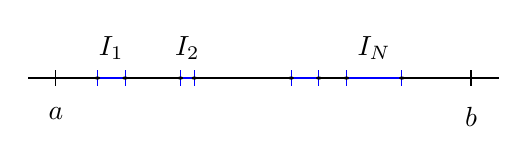
\begin{tikzpicture}[x=50]
       \draw (-1.2,0) -- (2.2,0);      
       \draw (-1, 0) node[below=7pt] {$a$};
       \draw[] (-1,-0.1) -- (-1,0.1);
       \draw (2, 0) node[below=7pt] {$b$};       
       \draw[] (2,-0.1) -- (2,0.1);
       
       \foreach \x in {-0.7,-0.5,-0.1,0, 0.7,0.9,1.1,1.5} {
        \draw[blue] (\x,-0.1) -- (\x,0.1);
    }
     \draw[blue, thick] (-0.7,0) -- (-0.5,0);
    \fill (-0.7,0) circle (0.02);
     \fill (-0.5,0) circle (0.02);
     
     \draw[blue, thick] (-0.1,0) -- (0,0);
    \fill (-0.1,0) circle (0.02);
     \fill (0,0) circle (0.02);
     
     \draw[blue, thick] (0.7,0) -- (0.9,0);
    \fill (0.7,0) circle (0.02);
     \fill (0.9,0) circle (0.02);
     
     \draw[blue, thick] (1.1,0) -- (1.5,0);
    \fill (1.1,0) circle (0.02);
     \fill (1.5,0) circle (0.02);
     
     \draw (-0.6, 0) node[above=3pt] {$I_1$};
     \draw (-0.05, 0) node[above=3pt] {$I_2$};
     \draw (1.3, 0) node[above=3pt] {$I_N$};
     
   \end{tikzpicture}$$

Con este recubrimiento finito, generamos una partición formada por $a$, $b$ y todos los extremos de los intervalos $I_j$ que denotaremos por $P$. Dicha partición, la expresaremos en términos de otras dos: $P_1$ que será la formada por los intervalos de la partición $P$ contenidos en algún $I_j$ y $P_2$ formada por los otros (que en particular no cortan a $D_{\varepsilon}$, luego la oscilación en estos es $<\varepsilon$). De este modo, tenemos $P = P_1 \cup P_2$.

Para cada intervalo $I\in P_2$, realizamos el siguiente procedimiento:
$$\forall I \in P_2:  \left(x \in I \Rightarrow o\left(f, x\right) < \varepsilon\right) \Rightarrow \exists I_x \subset I: \forall y, z \in I_x: \vert f\left(y\right) - f\left(z\right) \vert < \varepsilon$$
Y esto puede hacerse porque para cada $x$, podemos encontrar un $\delta$ de forma que en $(x-\delta, x+\delta)$ la oscilación es menor que $\varepsilon$ y precisamente ese sería un posible $I_x$.

Recubrimos $I$ (que es compacto por ser cerrado) por una cantidad finita de estos $I_x$ y, de esta manera, obtenemos en forma de partición (quitando trozos de intervalos si fuese necesario para que sean disjuntos) el intervalo $I$ inicial. Esto, genera otra partición de la parte que correspondía a $P_2$ que denotamos por $P^*_2$ y definimos $P^* := P_1 \cup P_2^*$ como nueva partición del intervalo.

De este modo, tenemos que:
$$U\left(f, P^* \right) - L\left(f, P^*\right) = \sum_{I\in P^*} \left(\sup_{x \in I} f \left(x\right) - \inf_{x \in I} f\left(x\right) \right) \mu\left(I\right) = $$
$$=\sum_{I \in P_1} \left( \sup_{x \in I} f \left(x\right) - \inf_{x \in I} f\left(x\right) \right) \mu\left(I\right) + \sum_{I \in P_2^*} \left(\sup_{x \in I} f \left(x\right) - \inf_{x \in I} f\left(x\right) \right) \mu\left(I\right) \le $$
$$ \leq 2M\varepsilon + \varepsilon\left(b - a\right) = \left(b - a + 2M\right) \varepsilon$$
Por el Criterio de Cauchy, $f$ es integrable Rienmann.

\item $\Rightarrow:$ supongamos que $f$ es integrable Riemann.

Como $D = \bigcup_{n \in \mathbb{N}} D_{\frac{1}{n}}$, basta con ver que $\forall n \in \mathbb{N}: \mu\left(D_{\frac{1}{n}}\right) = 0$. Para ello, tomamos $\varepsilon > 0$ y una partición $P$ de $\left[a, b\right]$ de forma que $U\left(f, P\right) - L\left(l, P\right) < \frac{\varepsilon}{n}$.

Denotamos por $P_1$ a los intervalos de $P$ que cortan a $D_{\frac{1}{n}}$ (con esto estamos asumiendo que los puntos de $D_{\frac{1}{n}}$ no son puntos de los extremos de la partición, pero no pasaría nada porque ese conjunto es de medida nula y la integral es la misma). De este modo, tenemos que:
$$\frac{\varepsilon}{n} > \sum_{I \in P_1} \left(\sup_{x \in I} f\left(x\right) - \inf_{x \in I} f\left(x\right) \right) \mu\left(I\right) \ge \frac{1}{n} \sum_{I \in P_1} \mu\left(I\right)$$
Sin embargo, esto quiere decir que:
$$\sum_{I \in P_1} \mu\left(I\right) < \varepsilon \mbox{ pero } D_{\frac{1}{n}} \subset \bigcup_{I \in P_1} I \Rightarrow \mu\left(D_{\frac{1}{m}}\right) = 0$$
\end{itemize}
\end{demo}

\begin{prop}
Si una función $f$ es integrable Riemann, entonces dicha función también es medible.
\end{prop}
\begin{demo}
Por el teorema de antes, $\mu(D) = 0$ lo que implica que $f$ es continua en c.t.p. y, por tanto, es medible.
\end{demo}

